
%% bare_conf.tex
%% V1.3
%% 2007/01/11
%% by Michael Shell
%% See:
%% http://www.michaelshell.org/
%% for current contact information.
%%
%% This is a skeleton file demonstrating the use of IEEEtran.cls
%% (requires IEEEtran.cls version 1.7 or later) with an IEEE conference paper.
%%
%% Support sites:
%% http://www.michaelshell.org/tex/ieeetran/
%% http://www.ctan.org/tex-archive/macros/latex/contrib/IEEEtran/
%% and
%% http://www.ieee.org/

%%*************************************************************************
%% Legal Notice:
%% This code is offered as-is without any warranty either expressed or
%% implied; without even the implied warranty of MERCHANTABILITY or
%% FITNESS FOR A PARTICULAR PURPOSE! 
%% User assumes all risk.
%% In no event shall IEEE or any contributor to this code be liable for
%% any damages or losses, including, but not limited to, incidental,
%% consequential, or any other damages, resulting from the use or misuse
%% of any information contained here.
%%
%% All comments are the opinions of their respective authors and are not
%% necessarily endorsed by the IEEE.
%%
%% This work is distributed under the LaTeX Project Public License (LPPL)
%% ( http://www.latex-project.org/ ) version 1.3, and may be freely used,
%% distributed and modified. A copy of the LPPL, version 1.3, is included
%% in the base LaTeX documentation of all distributions of LaTeX released
%% 2003/12/01 or later.
%% Retain all contribution notices and credits.
%% ** Modified files should be clearly indicated as such, including  **
%% ** renaming them and changing author support contact information. **
%%
%% File list of work: IEEEtran.cls, IEEEtran_HOWTO.pdf, bare_adv.tex,
%%                    bare_conf.tex, bare_jrnl.tex, bare_jrnl_compsoc.tex
%%*************************************************************************

% *** Authors should verify (and, if needed, correct) their LaTeX system  ***
% *** with the testflow diagnostic prior to trusting their LaTeX platform ***
% *** with production work. IEEE's font choices can trigger bugs that do  ***
% *** not appear when using other class files.                            ***
% The testflow support page is at:
% http://www.michaelshell.org/tex/testflow/



% Note that the a4paper option is mainly intended so that authors in
% countries using A4 can easily print to A4 and see how their papers will
% look in print - the typesetting of the document will not typically be
% affected with changes in paper size (but the bottom and side margins will).
% Use the testflow package mentioned above to verify correct handling of
% both paper sizes by the user's LaTeX system.
%
% Also note that the "draftcls" or "draftclsnofoot", not "draft", option
% should be used if it is desired that the figures are to be displayed in
% draft mode.
%
\documentclass[conference]{IEEEtran}
% Add the compsoc option for Computer Society conferences.
%
% If IEEEtran.cls has not been installed into the LaTeX system files,
% manually specify the path to it like:
% \documentclass[conference]{../sty/IEEEtran}





% Some very useful LaTeX packages include:
% (uncomment the ones you want to load)


% *** MISC UTILITY PACKAGES ***
%
%\usepackage{ifpdf}
% Heiko Oberdiek's ifpdf.sty is very useful if you need conditional
% compilation based on whether the output is pdf or dvi.
% usage:
% \ifpdf
%   % pdf code
% \else
%   % dvi code
% \fi
% The latest version of ifpdf.sty can be obtained from:
% http://www.ctan.org/tex-archive/macros/latex/contrib/oberdiek/
% Also, note that IEEEtran.cls V1.7 and later provides a builtin
% \ifCLASSINFOpdf conditional that works the same way.
% When switching from latex to pdflatex and vice-versa, the compiler may
% have to be run twice to clear warning/error messages.






% *** CITATION PACKAGES ***
%
%\usepackage{cite}
% cite.sty was written by Donald Arseneau
% V1.6 and later of IEEEtran pre-defines the format of the cite.sty package
% \cite{} output to follow that of IEEE. Loading the cite package will
% result in citation numbers being automatically sorted and properly
% "compressed/ranged". e.g., [1], [9], [2], [7], [5], [6] without using
% cite.sty will become [1], [2], [5]--[7], [9] using cite.sty. cite.sty's
% \cite will automatically add leading space, if needed. Use cite.sty's
% noadjust option (cite.sty V3.8 and later) if you want to turn this off.
% cite.sty is already installed on most LaTeX systems. Be sure and use
% version 4.0 (2003-05-27) and later if using hyperref.sty. cite.sty does
% not currently provide for hyperlinked citations.
% The latest version can be obtained at:
% http://www.ctan.org/tex-archive/macros/latex/contrib/cite/
% The documentation is contained in the cite.sty file itself.






% *** GRAPHICS RELATED PACKAGES ***
%
\ifCLASSINFOpdf
  % \usepackage[pdftex]{graphicx}
  % declare the path(s) where your graphic files are
  % \graphicspath{{../pdf/}{../jpeg/}}
  % and their extensions so you won't have to specify these with
  % every instance of \includegraphics
  % \DeclareGraphicsExtensions{.pdf,.jpeg,.png}
\else
  % or other class option (dvipsone, dvipdf, if not using dvips). graphicx
  % will default to the driver specified in the system graphics.cfg if no
  % driver is specified.
  % \usepackage[dvips]{graphicx}
  % declare the path(s) where your graphic files are
  % \graphicspath{{../eps/}}
  % and their extensions so you won't have to specify these with
  % every instance of \includegraphics
  % \DeclareGraphicsExtensions{.eps}
\fi
% graphicx was written by David Carlisle and Sebastian Rahtz. It is
% required if you want graphics, photos, etc. graphicx.sty is already
% installed on most LaTeX systems. The latest version and documentation can
% be obtained at: 
% http://www.ctan.org/tex-archive/macros/latex/required/graphics/
% Another good source of documentation is "Using Imported Graphics in
% LaTeX2e" by Keith Reckdahl which can be found as epslatex.ps or
% epslatex.pdf at: http://www.ctan.org/tex-archive/info/
%
% latex, and pdflatex in dvi mode, support graphics in encapsulated
% postscript (.eps) format. pdflatex in pdf mode supports graphics
% in .pdf, .jpeg, .png and .mps (metapost) formats. Users should ensure
% that all non-photo figures use a vector format (.eps, .pdf, .mps) and
% not a bitmapped formats (.jpeg, .png). IEEE frowns on bitmapped formats
% which can result in "jaggedy"/blurry rendering of lines and letters as
% well as large increases in file sizes.
%
% You can find documentation about the pdfTeX application at:
% http://www.tug.org/applications/pdftex





% *** MATH PACKAGES ***
%
%\usepackage[cmex10]{amsmath}
% A popular package from the American Mathematical Society that provides
% many useful and powerful commands for dealing with mathematics. If using
% it, be sure to load this package with the cmex10 option to ensure that
% only type 1 fonts will utilized at all point sizes. Without this option,
% it is possible that some math symbols, particularly those within
% footnotes, will be rendered in bitmap form which will result in a
% document that can not be IEEE Xplore compliant!
%
% Also, note that the amsmath package sets \interdisplaylinepenalty to 10000
% thus preventing page breaks from occurring within multiline equations. Use:
%\interdisplaylinepenalty=2500
% after loading amsmath to restore such page breaks as IEEEtran.cls normally
% does. amsmath.sty is already installed on most LaTeX systems. The latest
% version and documentation can be obtained at:
% http://www.ctan.org/tex-archive/macros/latex/required/amslatex/math/





% *** SPECIALIZED LIST PACKAGES ***
%
%\usepackage{algorithmic}
% algorithmic.sty was written by Peter Williams and Rogerio Brito.
% This package provides an algorithmic environment fo describing algorithms.
% You can use the algorithmic environment in-text or within a figure
% environment to provide for a floating algorithm. Do NOT use the algorithm
% floating environment provided by algorithm.sty (by the same authors) or
% algorithm2e.sty (by Christophe Fiorio) as IEEE does not use dedicated
% algorithm float types and packages that provide these will not provide
% correct IEEE style captions. The latest version and documentation of
% algorithmic.sty can be obtained at:
% http://www.ctan.org/tex-archive/macros/latex/contrib/algorithms/
% There is also a support site at:
% http://algorithms.berlios.de/index.html
% Also of interest may be the (relatively newer and more customizable)
% algorithmicx.sty package by Szasz Janos:
% http://www.ctan.org/tex-archive/macros/latex/contrib/algorithmicx/




% *** ALIGNMENT PACKAGES ***
%
%\usepackage{array}
% Frank Mittelbach's and David Carlisle's array.sty patches and improves
% the standard LaTeX2e array and tabular environments to provide better
% appearance and additional user controls. As the default LaTeX2e table
% generation code is lacking to the point of almost being broken with
% respect to the quality of the end results, all users are strongly
% advised to use an enhanced (at the very least that provided by array.sty)
% set of table tools. array.sty is already installed on most systems. The
% latest version and documentation can be obtained at:
% http://www.ctan.org/tex-archive/macros/latex/required/tools/


%\usepackage{mdwmath}
%\usepackage{mdwtab}
% Also highly recommended is Mark Wooding's extremely powerful MDW tools,
% especially mdwmath.sty and mdwtab.sty which are used to format equations
% and tables, respectively. The MDWtools set is already installed on most
% LaTeX systems. The lastest version and documentation is available at:
% http://www.ctan.org/tex-archive/macros/latex/contrib/mdwtools/


% IEEEtran contains the IEEEeqnarray family of commands that can be used to
% generate multiline equations as well as matrices, tables, etc., of high
% quality.


%\usepackage{eqparbox}
% Also of notable interest is Scott Pakin's eqparbox package for creating
% (automatically sized) equal width boxes - aka "natural width parboxes".
% Available at:
% http://www.ctan.org/tex-archive/macros/latex/contrib/eqparbox/





% *** SUBFIGURE PACKAGES ***
%\usepackage[tight,footnotesize]{subfigure}
% subfigure.sty was written by Steven Douglas Cochran. This package makes it
% easy to put subfigures in your figures. e.g., "Figure 1a and 1b". For IEEE
% work, it is a good idea to load it with the tight package option to reduce
% the amount of white space around the subfigures. subfigure.sty is already
% installed on most LaTeX systems. The latest version and documentation can
% be obtained at:
% http://www.ctan.org/tex-archive/obsolete/macros/latex/contrib/subfigure/
% subfigure.sty has been superceeded by subfig.sty.



%\usepackage[caption=false]{caption}
%\usepackage[font=footnotesize]{subfig}
% subfig.sty, also written by Steven Douglas Cochran, is the modern
% replacement for subfigure.sty. However, subfig.sty requires and
% automatically loads Axel Sommerfeldt's caption.sty which will override
% IEEEtran.cls handling of captions and this will result in nonIEEE style
% figure/table captions. To prevent this problem, be sure and preload
% caption.sty with its "caption=false" package option. This is will preserve
% IEEEtran.cls handing of captions. Version 1.3 (2005/06/28) and later 
% (recommended due to many improvements over 1.2) of subfig.sty supports
% the caption=false option directly:
%\usepackage[caption=false,font=footnotesize]{subfig}
%
% The latest version and documentation can be obtained at:
% http://www.ctan.org/tex-archive/macros/latex/contrib/subfig/
% The latest version and documentation of caption.sty can be obtained at:
% http://www.ctan.org/tex-archive/macros/latex/contrib/caption/




% *** FLOAT PACKAGES ***
%
%\usepackage{fixltx2e}
% fixltx2e, the successor to the earlier fix2col.sty, was written by
% Frank Mittelbach and David Carlisle. This package corrects a few problems
% in the LaTeX2e kernel, the most notable of which is that in current
% LaTeX2e releases, the ordering of single and double column floats is not
% guaranteed to be preserved. Thus, an unpatched LaTeX2e can allow a
% single column figure to be placed prior to an earlier double column
% figure. The latest version and documentation can be found at:
% http://www.ctan.org/tex-archive/macros/latex/base/



%\usepackage{stfloats}
% stfloats.sty was written by Sigitas Tolusis. This package gives LaTeX2e
% the ability to do double column floats at the bottom of the page as well
% as the top. (e.g., "\begin{figure*}[!b]" is not normally possible in
% LaTeX2e). It also provides a command:
%\fnbelowfloat
% to enable the placement of footnotes below bottom floats (the standard
% LaTeX2e kernel puts them above bottom floats). This is an invasive package
% which rewrites many portions of the LaTeX2e float routines. It may not work
% with other packages that modify the LaTeX2e float routines. The latest
% version and documentation can be obtained at:
% http://www.ctan.org/tex-archive/macros/latex/contrib/sttools/
% Documentation is contained in the stfloats.sty comments as well as in the
% presfull.pdf file. Do not use the stfloats baselinefloat ability as IEEE
% does not allow \baselineskip to stretch. Authors submitting work to the
% IEEE should note that IEEE rarely uses double column equations and
% that authors should try to avoid such use. Do not be tempted to use the
% cuted.sty or midfloat.sty packages (also by Sigitas Tolusis) as IEEE does
% not format its papers in such ways.





% *** PDF, URL AND HYPERLINK PACKAGES ***
%
%\usepackage{url}
% url.sty was written by Donald Arseneau. It provides better support for
% handling and breaking URLs. url.sty is already installed on most LaTeX
% systems. The latest version can be obtained at:
% http://www.ctan.org/tex-archive/macros/latex/contrib/misc/
% Read the url.sty source comments for usage information. Basically,
% \url{my_url_here}.

\usepackage{graphicx}
\usepackage[vlined,ruled]{algorithm2e}
\usepackage{xcolor}
\usepackage{listings}
\usepackage{listings-golang}
\usepackage{hyperref}




\definecolor{lightgray}{rgb}{.9,.9,.9}
\definecolor{darkgray}{rgb}{.4,.4,.4}
\definecolor{purple}{rgb}{0.65, 0.12, 0.82}
\definecolor{mygray}{rgb}{0.5,0.5,0.5}
\definecolor{mygreen}{rgb}{0,0.6,0}

\hypersetup{
    colorlinks,
    linkcolor={red},
    citecolor={blue},
    urlcolor={blue}
}

\lstset{ % add your own preferences
    basicstyle=\footnotesize,
    keywordstyle=\color{red},
    numbers=left,
    numbersep=5pt,
    showstringspaces=false, 
    stringstyle=\color{blue},
    tabsize=4,
    language=Golang % this is it !
}







% *** Do not adjust lengths that control margins, column widths, etc. ***
% *** Do not use packages that alter fonts (such as pslatex).         ***
% There should be no need to do such things with IEEEtran.cls V1.6 and later.
% (Unless specifically asked to do so by the journal or conference you plan
% to submit to, of course. )


% correct bad hyphenation here
\hyphenation{op-tical net-works semi-conduc-tor}


\begin{document}
%
% paper title
% can use linebreaks \\ within to get better formatting as desired
\title{Inferring Invariants of Distributed Programs}


% author names and affiliations
% use a multiple column layout for up to three different
% affiliations
\author{\IEEEauthorblockN{Keheliya Gallaba\IEEEauthorrefmark{1},
Arash Vahabzadeh\IEEEauthorrefmark{2}}
\IEEEauthorblockA{University of British Columbia\\
Vancouver, BC, Canada\\
Email: \IEEEauthorrefmark{1}kgallaba@ece.ubc.ca,
\IEEEauthorrefmark{2}arashvhb@ece.ubc.ca}}

% conference papers do not typically use \thanks and this command
% is locked out in conference mode. If really needed, such as for
% the acknowledgment of grants, issue a \IEEEoverridecommandlockouts
% after \documentclass

% for over three affiliations, or if they all won't fit within the width
% of the page, use this alternative format:
% 
%\author{\IEEEauthorblockN{Michael Shell\IEEEauthorrefmark{1},
%Homer Simpson\IEEEauthorrefmark{2},
%James Kirk\IEEEauthorrefmark{3}, 
%Montgomery Scott\IEEEauthorrefmark{3} and
%Eldon Tyrell\IEEEauthorrefmark{4}}
%\IEEEauthorblockA{\IEEEauthorrefmark{1}School of Electrical and Computer Engineering\\
%Georgia Institute of Technology,
%Atlanta, Georgia 30332--0250\\ Email: see http://www.michaelshell.org/contact.html}
%\IEEEauthorblockA{\IEEEauthorrefmark{2}Twentieth Century Fox, Springfield, USA\\
%Email: homer@thesimpsons.com}
%\IEEEauthorblockA{\IEEEauthorrefmark{3}Starfleet Academy, San Francisco, California 96678-2391\\
%Telephone: (800) 555--1212, Fax: (888) 555--1212}
%\IEEEauthorblockA{\IEEEauthorrefmark{4}Tyrell Inc., 123 Replicant Street, Los Angeles, California 90210--4321}}




% use for special paper notices
%\IEEEspecialpapernotice{(Invited Paper)}




% make the title area
\maketitle


% \begin{abstract}
% %\boldmath
% The abstract goes here.
% \end{abstract}
% IEEEtran.cls defaults to using nonbold math in the Abstract.
% This preserves the distinction between vectors and scalars. However,
% if the conference you are submitting to favors bold math in the abstract,
% then you can use LaTeX's standard command \boldmath at the very start
% of the abstract to achieve this. Many IEEE journals/conferences frown on
% math in the abstract anyway.

% no keywords




% For peer review papers, you can put extra information on the cover
% page as needed:
% \ifCLASSOPTIONpeerreview
% \begin{center} \bfseries EDICS Category: 3-BBND \end{center}
% \fi
%
% For peerreview papers, this IEEEtran command inserts a page break and
% creates the second title. It will be ignored for other modes.
\IEEEpeerreviewmaketitle



\section{Introduction}

Building a reliable distributed system is a difficult task, since
distributed system should continue operating even when components or
network fail, this means that there are many corner cases that
developers should consider when building the system. Building such a
reliable and dependable system is not possible without thorough
testing of the system. But unfortunately testing a distributed system
is a much more difficult task because it is much harder to test
components of a distributed system in isolation. There are many
failure scenarios that distributed system should handle and these
scenarios should be tested as well. In some cases reproducing the
failures is a difficult task e.g. degrading network performance for
test purposes. Many bugs turn out to be heisenbugs in distributed
system which are hard to reproduce and detect. For testing and
debugging distributed systems, developers and testers have to spend a
considerable amount of time inspecting logs of the system manually and
looking for incidents that system does not behave as expected. One
alternative to this laborious approach is to define invariants for
system’s expected behaviour and check the software traces against
these invariants. This approach is considerably easier than the former
but as the system gets larger and more complex, providing invariants
manually becomes more difficult.

Testing distributed systems is hard because a fault in a single node
does not confine to that node, instead it may cause an error in
another node. In fact errors in distributed system should be defined
on global state of the system not a single node. In this work we
assume that state of each node is comprised of its variables. Not all
variables of one node is affected by other nodes, we define the set of
variables of one node whose values are affected by other nodes as
distributed state of that node. We refer to set of distributed state
of all nodes as distributed state of the system.


Our approach is to automatically infer invariants that may exist in
distributed state of our system. To this end, we execute distributed
programs and dynamically select a set of variables in each node that
likely represent the distributed state across our distributed nodes.
We do so with dynamic data flow analysis of variables and selecting
those that are affected by a send or receive operation. Finally we use
Daikon to infer invariants among our distributed state variables.

%We are going to find invariants in distributed programs
%For that we need to find distributed state



\section{Approach}

The ultimate goal of this project is to infer invariants in a
distributed system. For the scope of this project we will consider a system with 2 nodes. Before inferring invariants we need to identify likely distributed
state variables. We define distributed state variables, as variables
that are stored in one node whose values are affected or determined by
the other remote node in the distributed system. It should be noted that
these variables are only a part of the state in a distributed system
at a given time. For our case we assume that these capture a
significant portion of the state. Consider the code samples
Listing~\ref{lst:node0} and Listing~\ref{lst:node1} showing the
communication between two nodes in a distributed system. The
communication between the nodes can be depicted as shown in
Figure~\ref{fig:sample_code_diag}. We need to infer the equality
between elements in each pair \texttt{(a,first),
(b,second),(sum,result)} and also the properites: \texttt{(result = a
+ b)} and \texttt{(sum = first + second)}.


\begin{figure}
  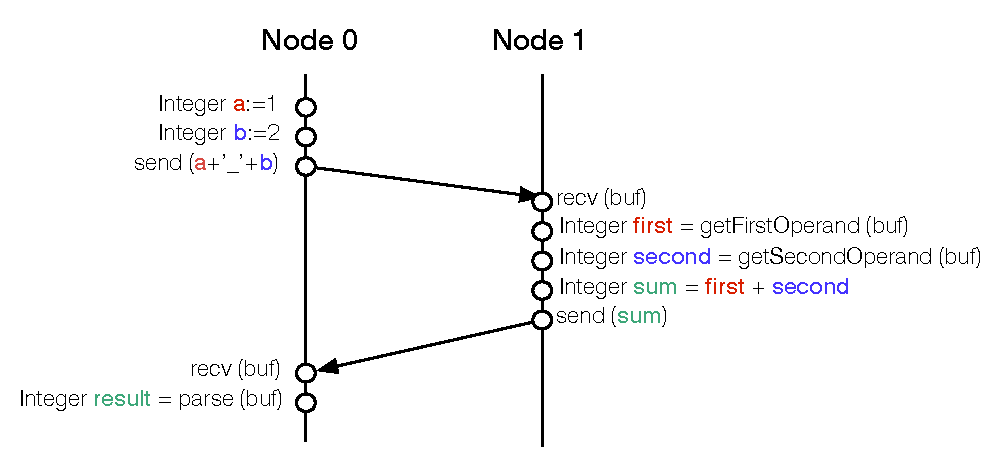
\includegraphics[width=\columnwidth]{sample_code.pdf}
  \caption{Example communication between two nodes in a distributed system}
  \label{fig:sample_code_diag}
\end{figure}

\begin{figure}
\begin{lstlisting}[caption={Sample code for Communication between 2 nodes - Node 0}, label=lst:node0]
    Integer a := 1
    Integer b := 2
    send ( a + '_' + b )
    recv (buf)
    Integer result := parse (buf)
\end{lstlisting}
\end{figure}

\begin{figure}
\begin{lstlisting}[caption={Sample code for Communication between 2 nodes - Node 1}, label=lst:node1]
    recv (buf)
    Integer first := getFirstOperand( buf )
    Integer second := getSecondOperand( buf )
    Integer sum := first + second
    send ( sum )
\end{lstlisting}
\end{figure}

The naive approach for inferring these invariants will be to dump all
state varaible values at all program points and feed them to an
invariant detector like daikon\cite{ernst2007daikon}. But given the
number of program points and huge number of variables in a relatively
large program this approach is not scalable. So we propose 2 main
optimizations to reduce the number of program point, variable value
combinations.

\subsection{Detecting interesting program points}

Rather than dumping state at all program points we expect the
developer to mark interesting program points using annotations. The
program state will be dumped at only these annotated points. This will
also help to narrow down the focus to points that are identified by
the developer as interesting points without wasting resources
analyzing useless program points. The annotations will be identified
by the parser at the instrumentation phase and re-written to include
statements which will write the values of variable to a file when the
program reaches that point in the runtime.

\subsection{Dataflow analysis for Go programs}

Even at interesting program points, variable space that need to be
captured is very large. So only the variables that were affected by
the communication with other nodes need to be identified. To detect
these variables, some form of dataflow analysis is required. This
includes the dataflow of the distributed system as a whole and also in
a single program. But currently there are no data flow analysis
frameworks available for Go programs.

This is a challenging problem in itself because Go language has
special constructs like channels to share data between goroutines. We
are planning to do this analysis dynamically by instrumenting variable
declarations and assignments, and then collecting execution traces of
each of these statements. We have chosen this approach because it
gives information about the actual execution and therefore is more
accurate. For this we are hoping to use static analysis libraries
available under Go-lang tools\cite{static_golang} which provide
support for Identifier resolution, Type information, Call graph
navigation and Channel peers (send $\leftrightarrow$ receive)
identification.

Our dynamic dataflow analysis is focused on mainly providing the
following features. Given a variable, start line and end line it will
return a set of variables affected by that variable between start line
and the end line.

As the next phase of our project, using the above analysis, we hope to
find out variables affected by receiving messages in interprocess
communication channels like RPC and TCP/UDP sockets. We will get the
values of these variables just before another send/receive or end of
function whichever occurs first. We assume these set of variables at
the send statement in both (sending and receiving) nodes taken
together represent global state of the distributed system.

Given two nodes which are communicating we have two such sets of
variables representing a particular state. So we will select the
corresponding variable pairs from send and receive of each node
mentioned in the previous step and provide as inputs for the Daikon
invariant detector. This will give us a set of properties that were
true over the observed executions across 2 nodes. Overall execution
flow of the analysis is shown in Figure~\ref{fig:go_flow}.


\begin{figure}
  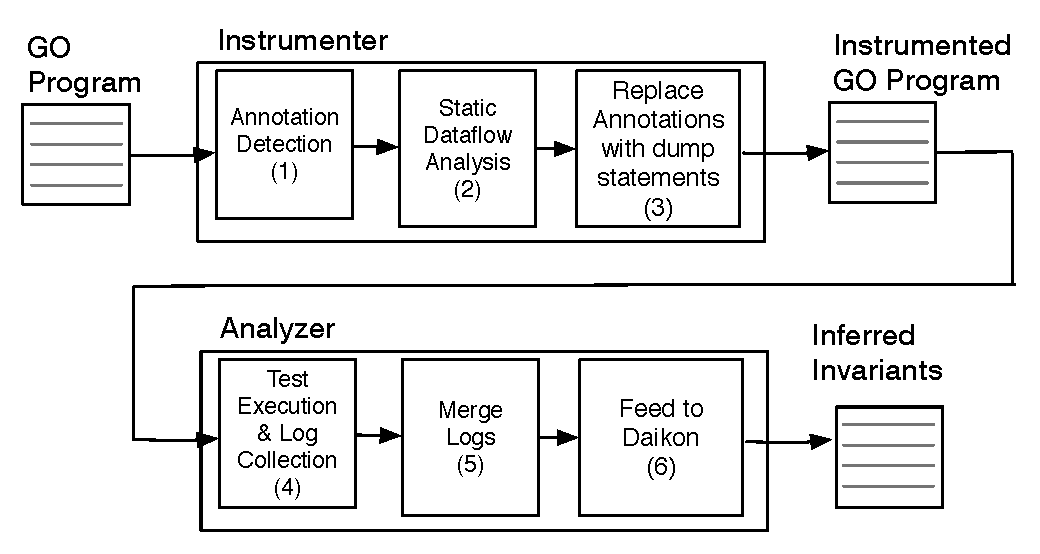
\includegraphics[width=\columnwidth]{go_flow.pdf}
  \caption{Flow of the invariant inference of Go programs}
  \label{fig:go_flow}
\end{figure}

\subsection{Timeline}

\section{Related Work}

Yabandeh et al.\cite{yabandeh2011finding} proposed an approach to
infer almost-invariants in distributed systems. They infer the
invariants that are true in most cases and assume these invariants
only get violated due to manifestation of bugs. There are a number of
ways our approach differ from theirs: Their approach requires user to
provide a list of variables and functions that they want to consider
for inferring invariants while our approach infers distributed state
variables automatically. Moreover, they assume that an external module
generates a trace of globally consistent state system for their
algorithm while our approach extract these states through dynamic
execution of the distributed system.

Ernst et al.\cite{ernst2001dynamically} infer invariants in a
sequential program by executing the program on a collection of inputs.
This invariant detector has been released as a tool called
Daikon\cite{ernst2007daikon}. Although, we use their tool to infer
invariants, detecting invariants in a distributed system poses unique
challenges to identify distributed state and valid global states among
a larger set of variables. Ne Win et al.\cite{NeWinEGKL04} use daikon
to assist theorem provers for verifying distributed algorithms. To
demonstrate their approach, they proved the correctness of the Paxos
algorithm.


%2 daikon : I do not know how to describe other paper because they are basically the same
%almost-invariant
%paxos proving using dykon

% trigger a \newpage just before the given reference
% number - used to balance the columns on the last page
% adjust value as needed - may need to be readjusted if
% the document is modified later
%\IEEEtriggeratref{8}
% The "triggered" command can be changed if desired:
%\IEEEtriggercmd{\enlargethispage{-5in}}

% references section

% can use a bibliography generated by BibTeX as a .bbl file
% BibTeX documentation can be easily obtained at:
% http://www.ctan.org/tex-archive/biblio/bibtex/contrib/doc/
% The IEEEtran BibTeX style support page is at:
% http://www.michaelshell.org/tex/ieeetran/bibtex/
%\bibliographystyle{IEEEtran}
% argument is your BibTeX string definitions and bibliography database(s)
%\bibliography{IEEEabrv,../bib/paper}
%
% <OR> manually copy in the resultant .bbl file
% set second argument of \begin to the number of references
% (used to reserve space for the reference number labels box)
%\begin{thebibliography}{1}

\bibliographystyle{IEEEtran}
\bibliography{paper}
% \bibitem{IEEEhowto:kopka}
% H.~Kopka and P.~W. Daly, \emph{A Guide to \LaTeX}, 3rd~ed.\hskip 1em plus
%   0.5em minus 0.4em\relax Harlow, England: Addison-Wesley, 1999.
%\end{thebibliography}




% that's all folks
\end{document}


